\chapter{Methods and experiments}

This chapter aims to describe the evaluation methods of the KubeFold platform on the AWS cloud and discuss the computation results.

\section{Runtime environment}

The previous chapter described the architecture and implementation of the KubeFold project.
The final result is a set of three executable files that must be run in a cluster.
Each of them was placed in a container image, and the images were pushed to the GitHub Container Registry (\textit{ghcr.io})~\cite{ghcr}.
To run the project, a temporary Kubernetes cluster was set up, on which the operator was installed along with its components.

%TODO jakis opis kontekstu zanim sie powie o tym, e trzeba uruchomic eksctl - co wyporodukowalismy w poprzednim rozdziale, co nam daje AWS, co i po co uruchamiamy, jak instalujemy, gdzie i jak ladujey dane wsadowe etc.
The project was run on the AWS EKS platform~\ref{subsec:aws-eks}.
AWS EKS is a managed service for running Kubernetes clusters without the need to configure key Kubernetes platform components such as Control Plane, which are difficult to install.
This is one of the options for running a cluster, but it would also be possible to set up a cluster locally or on a bare-metal server.
The \texttt{eksctl} tool was used to quickly launch the cluster, with the cluster configured in the \texttt{eu-central-1} region with two node groups - CPU and GPU.
The configuration is shown in listing~\ref{lst:eksctl}.
It's worth noting the attached AWS IAM policies that grant permissions for node groups to services such as AWS S3, AWS SNS, and AWS FSx.

\begin{lstlisting}[language=yaml,caption={\texttt{eksctl} configuration used for launching AWS EKS cluster},label={lst:eksctl}]
apiVersion: eksctl.io/v1alpha5
kind: ClusterConfig
metadata:
  name: alphafold-cluster
  region: eu-central-1

managedNodeGroups:
  - name: ng-primary # Cheaper node group without GPU devices
    instanceType: m5.xlarge
    desiredCapacity: 1
    subnets:
      - "subnet-038b10f6f4ac5aacd"
    iam:
      withAddonPolicies:
        ebs: true
        fsx: true
        efs: true
      attachPolicyARNs:
        - arn:aws:iam::aws:policy/AmazonEKSWorkerNodePolicy
        - arn:aws:iam::aws:policy/AmazonEKS_CNI_Policy
        - arn:aws:iam::aws:policy/AmazonFSxFullAccess
        - arn:aws:iam::aws:policy/AmazonS3FullAccess
        - arn:aws:iam::aws:policy/AmazonSNSFullAccess
        - arn:aws:iam::aws:policy/AmazonEC2ContainerRegistryReadOnly
        - arn:aws:iam::aws:policy/AmazonSSMManagedInstanceCore
  - name: ng-gpu # More expensive node group with GPU devices
    instanceType: g5.xlarge
    desiredCapacity: 1
    subnets:
      - "subnet-038b10f6f4ac5aacd"
    iam:
      withAddonPolicies:
        ebs: true
        fsx: true
        efs: true
      attachPolicyARNs:
        - arn:aws:iam::aws:policy/AmazonEKSWorkerNodePolicy
        - arn:aws:iam::aws:policy/AmazonEKS_CNI_Policy
        - arn:aws:iam::aws:policy/AmazonFSxFullAccess
        - arn:aws:iam::aws:policy/AmazonS3FullAccess
        - arn:aws:iam::aws:policy/AmazonSNSFullAccess
        - arn:aws:iam::aws:policy/AmazonEC2ContainerRegistryReadOnly
        - arn:aws:iam::aws:policy/AmazonSSMManagedInstanceCore

iam:
  withOIDC: true
  serviceAccounts:
    - metadata:
        name: fsx-csi-controller-sa
        namespace: kube-system
        labels: { aws-usage: "application" }
      attachPolicyARNs:
        - "arn:aws:iam::aws:policy/AmazonFSxFullAccess"

vpc:
  id: vpc-0ade33da149682ec2
  subnets:
    public:
      eu-central-1a:
        id: "subnet-038b10f6f4ac5aacd"
      eu-central-1b:
        id: "subnet-099b2b55ca156bb7d"

addons:
  - name: vpc-cni
  - name: coredns
  - name: kube-proxy
  - name: eks-pod-identity-agent
\end{lstlisting}

On the cluster, the AWS FSx CSI Driver has been installed.
It is used for automatic creation and management of AWS FSx for Lustre volumes based on \texttt{PersistentVolumeClaim} resources created in the cluster.
To make this possible, it is necessary to configure a \texttt{StorageClass} that specifies how volumes should be created.
In the configuration shown in listing~\ref{lst:storage-class}, parameters such as file system version, compression type (disabled), volume throughput, and network settings were defined.
This means that creating a \texttt{PersistentVolumeClaim} resource pointing to the \texttt{StorageClass} named \texttt{fsx-sc} will automatically provision a new FSx file system in AWS.

\begin{lstlisting}[language=yaml,caption={Definition of \texttt{StorageClass} for FSx CSI Driver},label={lst:storage-class}]
kind: StorageClass
apiVersion: storage.k8s.io/v1
metadata:
  name: fsx-sc
provisioner: fsx.csi.aws.com
parameters:
  subnetId: subnet-038b10f6f4ac5aacd
  securityGroupIds: sg-058c31d84bfd004cf,sg-04e79090b86912eae,sg-07d7ceb3fa050568c,sg-02a2a067c7f724318
  deploymentType: PERSISTENT_1
  perUnitStorageThroughput: "200"
  dataCompressionType: "NONE"
  fileSystemTypeVersion: "2.15"
\end{lstlisting}

The KubeFold operator was installed using the installation file generated by the KubeBuilder tool.
It is located in the GitHub code repository under the path \texttt{dist/install.yaml}.
The installation therefore comes down to executing a single command: \texttt{kubectl apply -f https://raw.githubusercontent.com/kubefold/operator/ \n refs/heads/main/dist/install.yaml}.
This makes it very fast and convenient from the administrator's perspective.

\begin{lstlisting}[language=bash,caption={Quick project startup script},label={lst:up-script}]
#!/bin/bash

export AWS_PAGER=""
ACCOUNT_ID=$(aws sts get-caller-identity --query Account --output text)
eksctl create cluster -f eks/cluster.yaml
aws eks update-kubeconfig --name alphafold-cluster --region eu-central-1
kubectl config use-context arn:aws:eks:eu-central-1:"$ACCOUNT_ID":cluster/alphafold-cluster
kubectl apply -k "github.com/kubernetes-sigs/aws-fsx-csi-driver/deploy/kubernetes/overlays/stable/?ref=release-1.3"
kubectl apply -f eks/fsx.storageclass.k8s.yaml

kubectl apply -f https://raw.githubusercontent.com/kubefold/operator/refs/heads/main/dist/install.yaml
kubectl apply -f config/samples/data_v1_proteindatabase.yaml

echo 'Done'
\end{lstlisting}

A \texttt{up.sh} script was prepared for quickly setting up the environment with all necessary dependencies, which is shown in listing~\ref{lst:up-script}.
After executing the script, you can directly proceed to start working with KubeFold.
%To trzeba lepoej omowic co jest na screenie - jak sprawdzic, ze jest ok etc.
If the setup was installed correctly, running the command:\newline
\texttt{kubectl get pods -A} \newline
should show output similar to that in screenshot~\ref{fig:eks_pods_terminal}.
The screenshot shows a pod named \texttt{kubefold-controller-manager-55bdf77c8c-wwhl2} in the \texttt{kubefold-system} namespace, and the cluster reports that all pods are \textit{Ready}.
This means that the operator has been successfully launched and has successfully connected to the Kubernetes API server.

\begin{figure}[htbp]
    \centering
    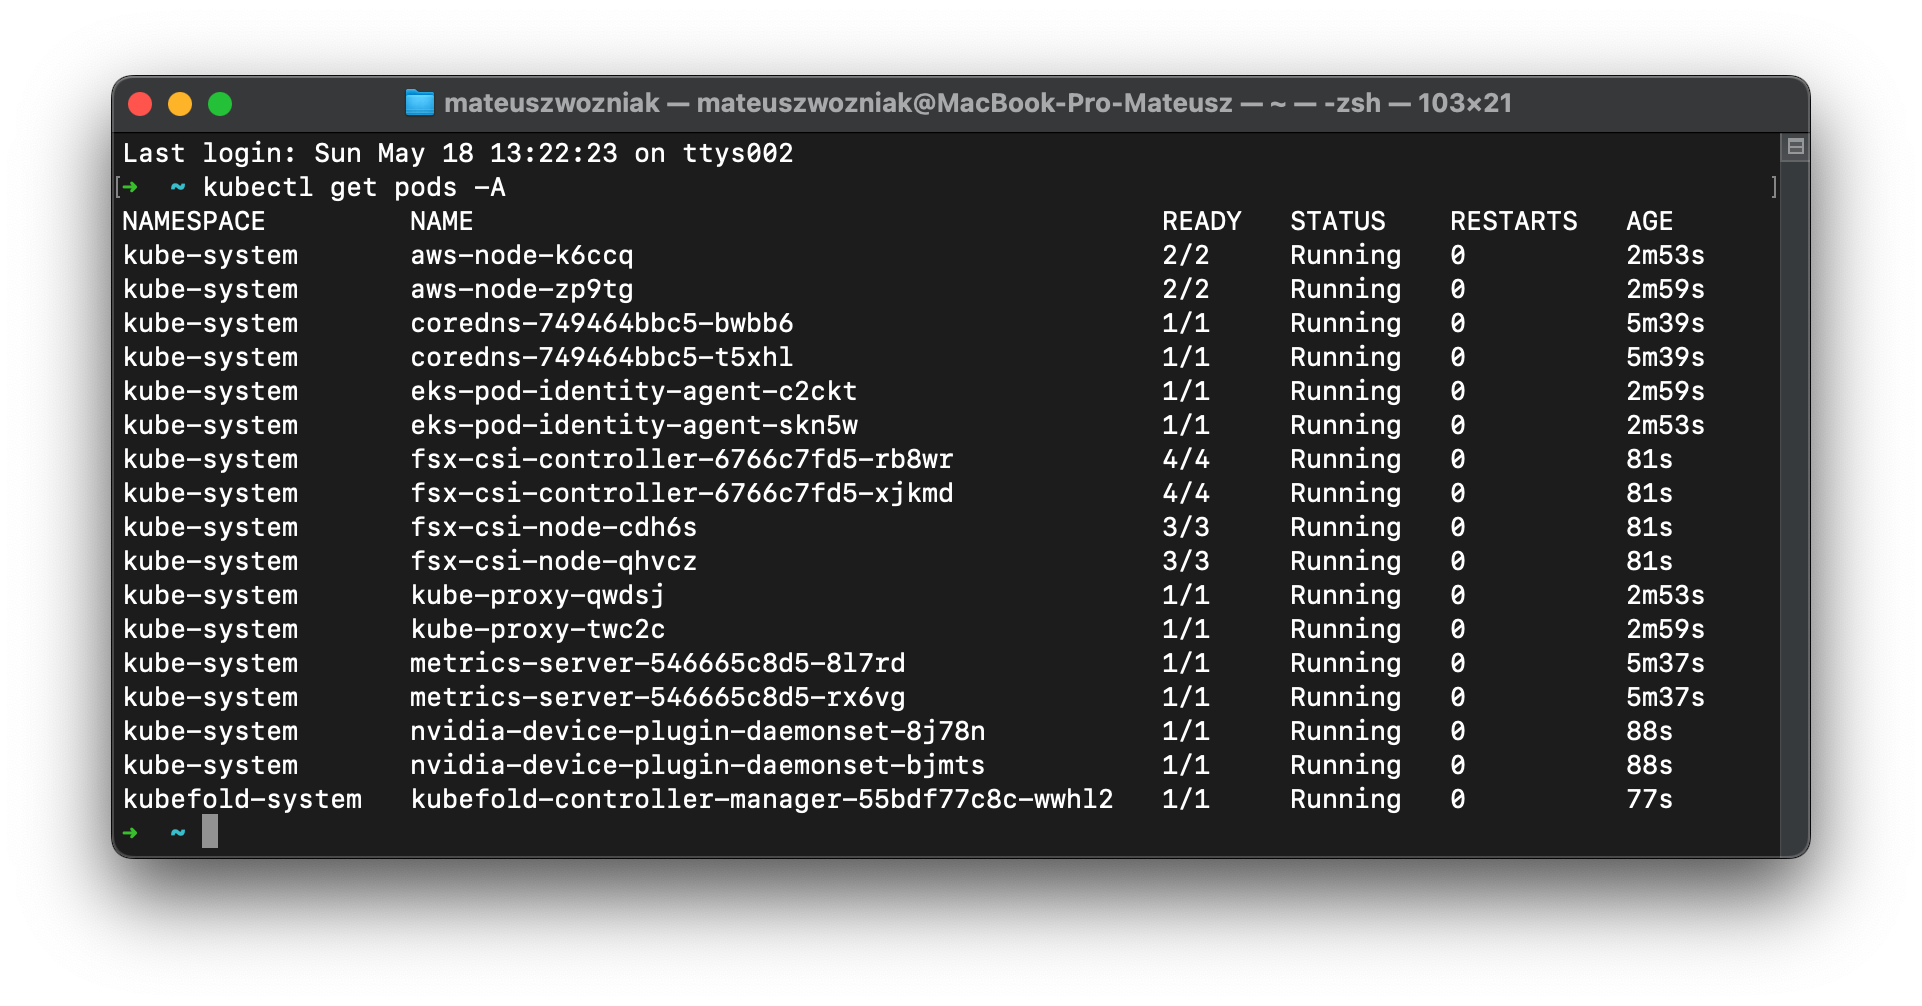
\includegraphics[width=\textwidth]{images/eks_pods_terminal}
    \caption{Command \texttt{kubectl get pods} output after successful cluster installation}
    \label{fig:eks_pods_terminal}
\end{figure}

\section{Prepared resource definitions}

The following YAML resource definitions were prepared for testing KubeFold.
The first one is the \texttt{ProteinDatabase} resource shown in listing~\ref{lst:used_protein_database}.
The second one is the \texttt{ProteinConformationPrediction} resource shown in listing~\ref{lst:used_protein_conformation_prediction}.
Both resources were applied to the cluster using \texttt{kubectl apply} right after installation.

\begin{lstlisting}[language=yaml,caption={Used \texttt{ProteinDatabase} resource definition},label={lst:used_protein_database}]
apiVersion: data.kubefold.io/v1
kind: ProteinDatabase
metadata:
  name: proteindatabase-sample
spec:
  datasets:
    bfd: true
    mgyclusters: true
    nt: true
    pdb: true
    pdbseqreq: true
    rfam: true
    rnacentral: true
    uniref90: true
    uniprot: true
  volume:
    storageClassName: fsx-sc
\end{lstlisting}

\begin{lstlisting}[language=yaml,caption={Used \texttt{ProteinConformationPrediction} resource definition},label={lst:used_protein_conformation_prediction}]
apiVersion: data.kubefold.io/v1
kind: ProteinConformationPrediction
metadata:
  name: proteinconformationprediction-sample
spec:
  database: proteindatabase-sample
  protein:
    id: [ 'A','B' ]
    sequence: GMRESY...LQQANDLKQG
  model:
    volume:
      storageClassName: fsx-sc
    weights:
      http: https://staticfilehosting.com/af3.bin.zst
    seeds:
      - 1
  destination:
    s3:
      bucket: kubefold-artifacts-sample
      region: eu-central-1
  notify:
    region: eu-central-1
    sms:
      - "+48140690323"
\end{lstlisting}.

When the \texttt{ProteinDatabase} resource was created, the FSx CSI Driver triggered the creation of an FSx for Lustre file system (see fig.~\ref{fig:fsx_fs}).
As soon as the file system was created, the process of downloading protein databases began in multiple pods simultaneously.
The user can monitor the download progress in real-time, as shown in screenshot~\ref{fig:used_proteindatabase_terminal}.
After the download is complete, the status will be changed to \textit{Completed} (see screenshot~\ref{fig:proteindatabase_completed_terminal}).

\begin{figure}[htbp]
    \centering
    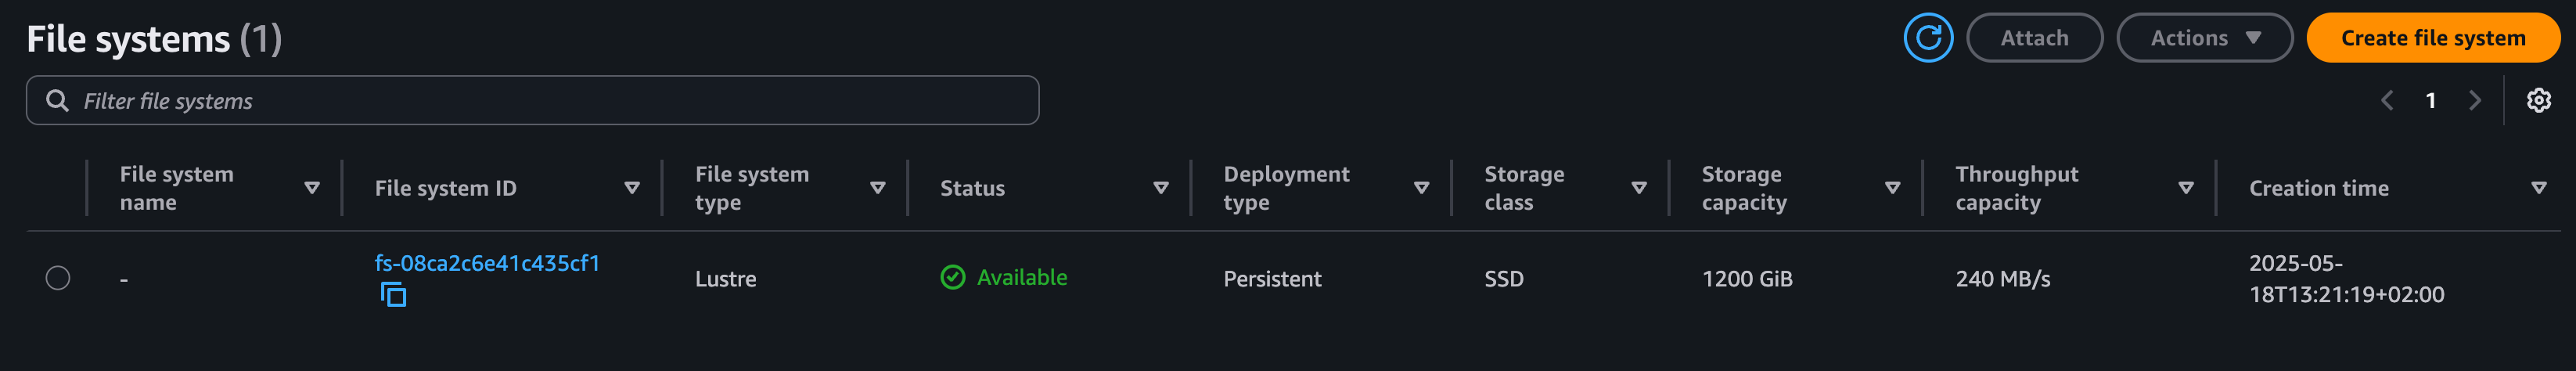
\includegraphics[width=\textwidth]{images/fsx_fs}
    \caption{Created FSx for Lustre file system in AWS Web Console}
    \label{fig:fsx_fs}
\end{figure}

\begin{figure}[htbp]
    \centering
    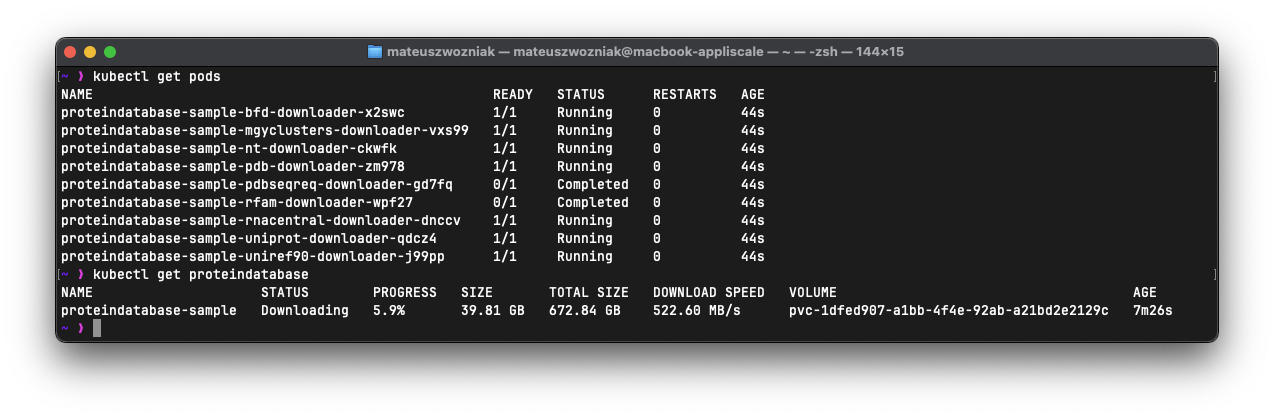
\includegraphics[width=\textwidth]{images/old_proteindatabase_terminal}
    \caption{Terminal output presenting \texttt{ProteinDatabase} resource}
    \label{fig:used_proteindatabase_terminal}
\end{figure}

\begin{figure}[htbp]
    \centering
    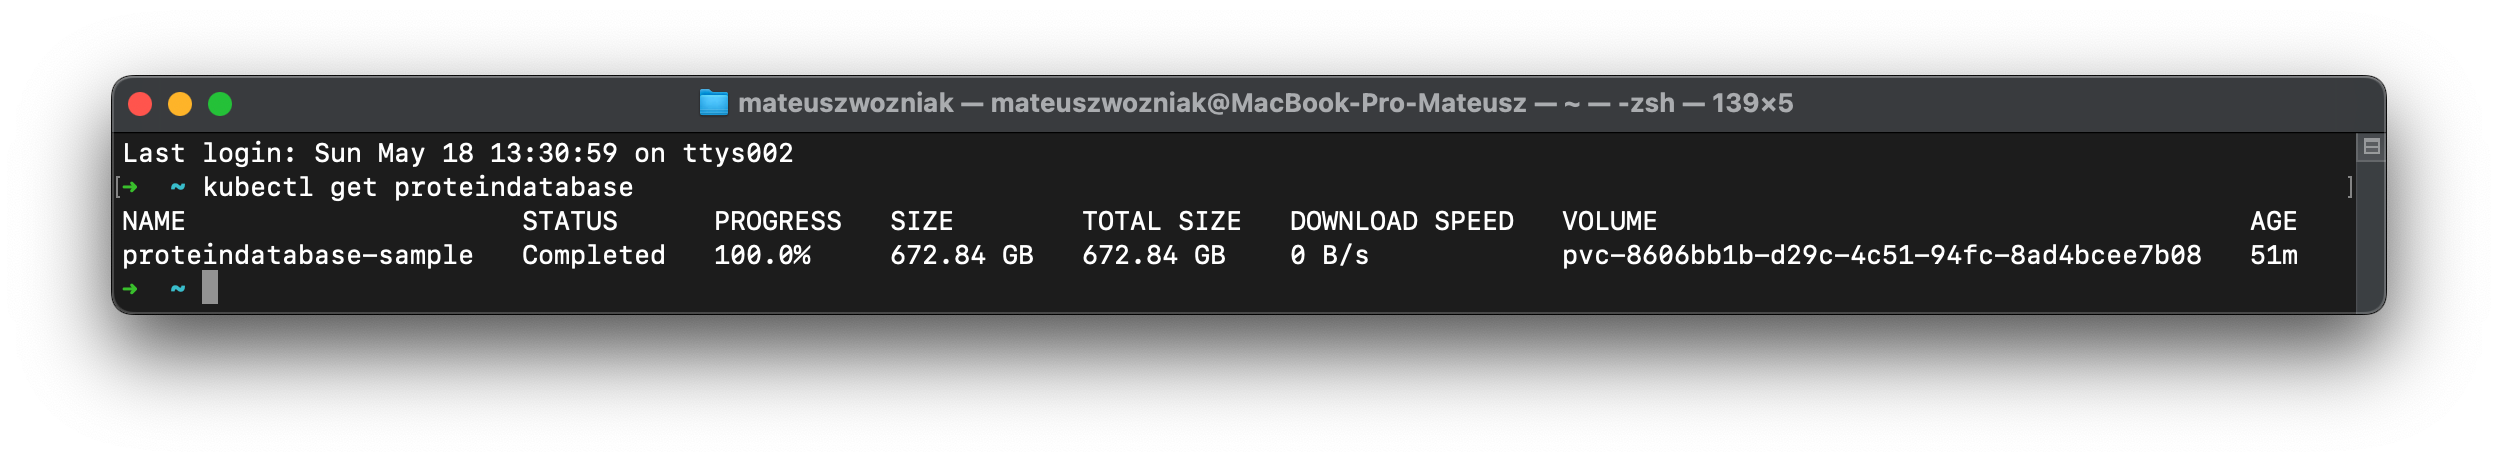
\includegraphics[width=\textwidth]{images/proteindatabase_completed_terminal}
    \caption{Completed downloading of protein database}
    \label{fig:proteindatabase_completed_terminal}
\end{figure}

After applying the \texttt{ProteinConformationPrediction} resource, the KubeFold operator launches three Jobs in sequence, corresponding to three phases of the task.
The initial phase is the \textit{Aligning} phase, which the user can check by running the \texttt{kubectl get proteinconformationprediction} command in the terminal (see screenshot~\ref{fig:proteinconformationprediction_aligning_terminal}). It launches a pod with the \texttt{-search} suffix on a node equipped with large CPU resources.

The second phase is the \textit{Predicting} phase (terminal output is shown in screenshot~\ref{fig:proteinconformationprediction_predicting_terminal}), which runs on a node equipped with a tensor computation accelerator such as GPU or TPU.
In this phase, the pod was created with the \texttt{-predict} suffix.

The final phase is the \texttt{UploadingArtifacts} phase, which is responsible for sending computation artifacts to AWS S3 storage and queuing notifications to research team members (see screenshot~\ref{fig:proteinconformationprediction_uploading_terminal}). When this step is completed, the status will be changed to \texttt{Completed} (see screenshot~\ref{fig:proteindatabase_completed_terminal}).

\begin{figure}[htbp]
    \centering
    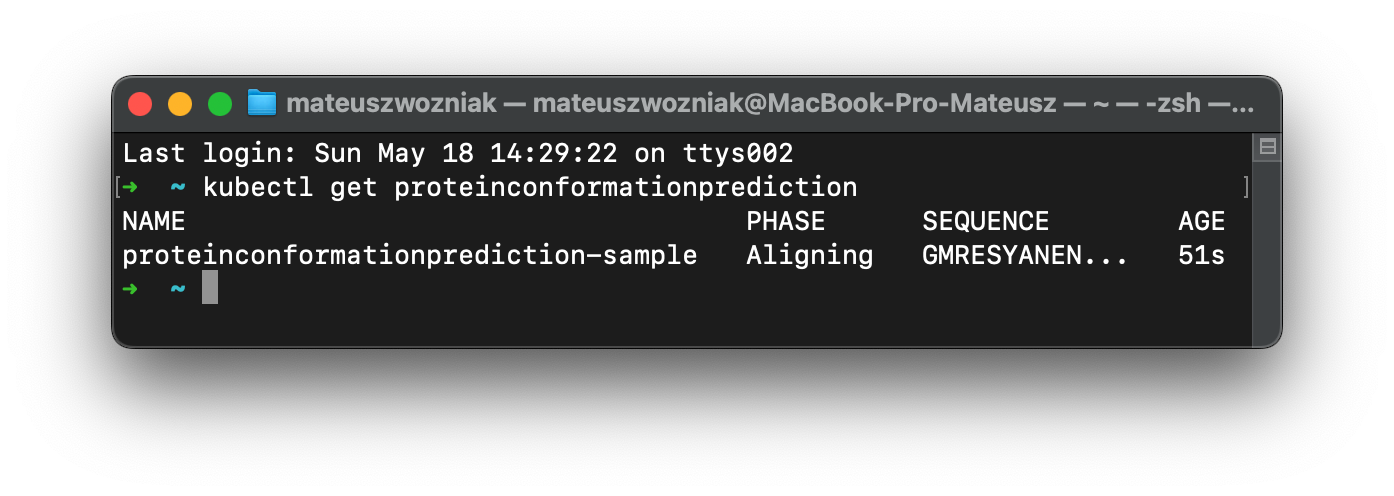
\includegraphics[width=\textwidth]{images/proteinconformationprediction_aligning_terminal}
    \caption{Aligning phase in protein conformation prediction task}
    \label{fig:proteinconformationprediction_aligning_terminal}
\end{figure}

\begin{figure}[htbp]
    \centering
    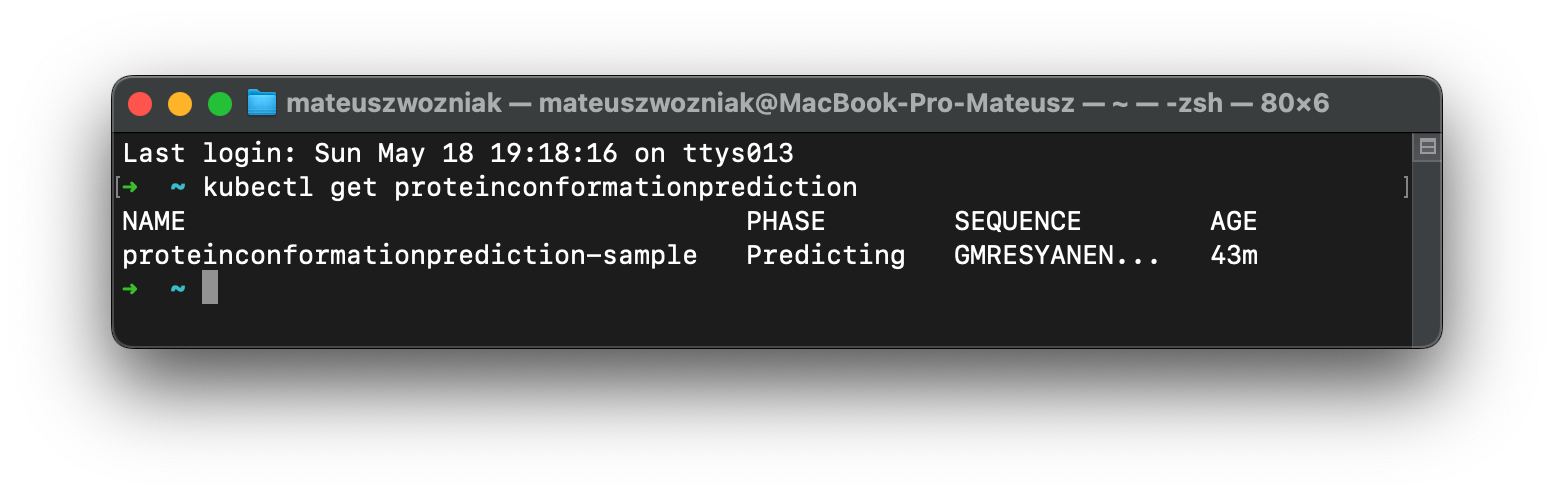
\includegraphics[width=\textwidth]{images/proteinconformationprediction_predicting_terminal}
    \caption{Predicting phase in protein conformation prediction task}
    \label{fig:proteinconformationprediction_predicting_terminal}
\end{figure}

\begin{figure}[htbp]
    \centering
    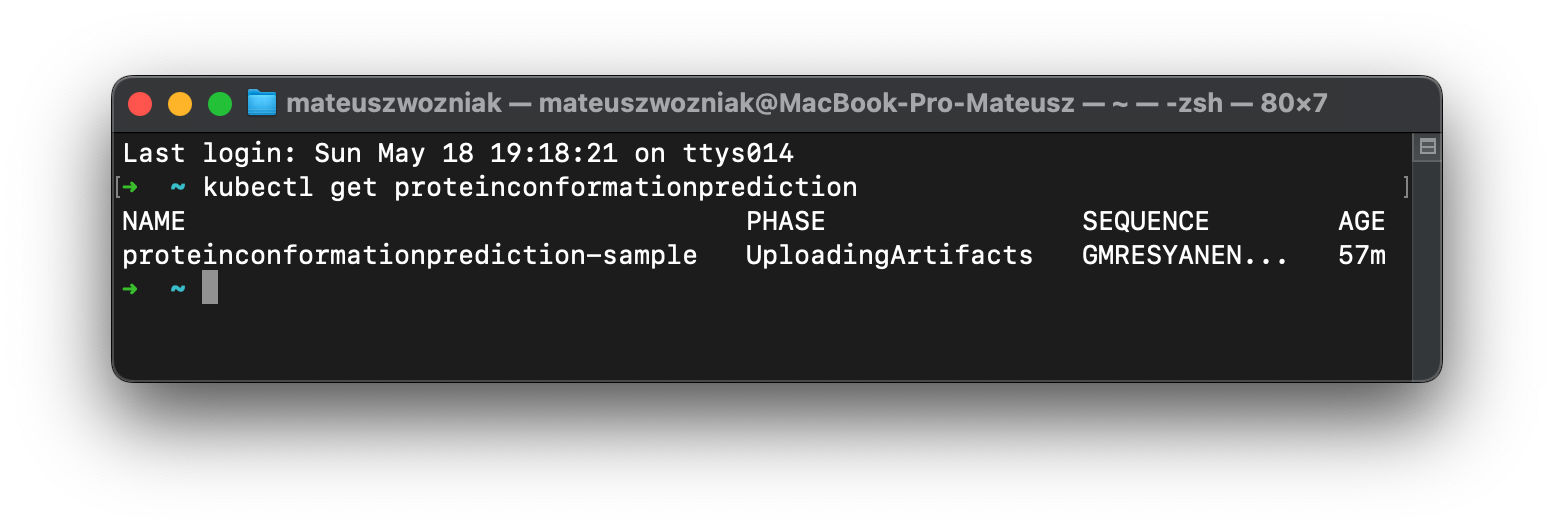
\includegraphics[width=\textwidth]{images/proteinconformationprediction_uploading_terminal}
    \caption{Post processing phase in protein conformation prediction task}
    \label{fig:proteinconformationprediction_uploading_terminal}
\end{figure}

\begin{figure}[htbp]
    \centering
    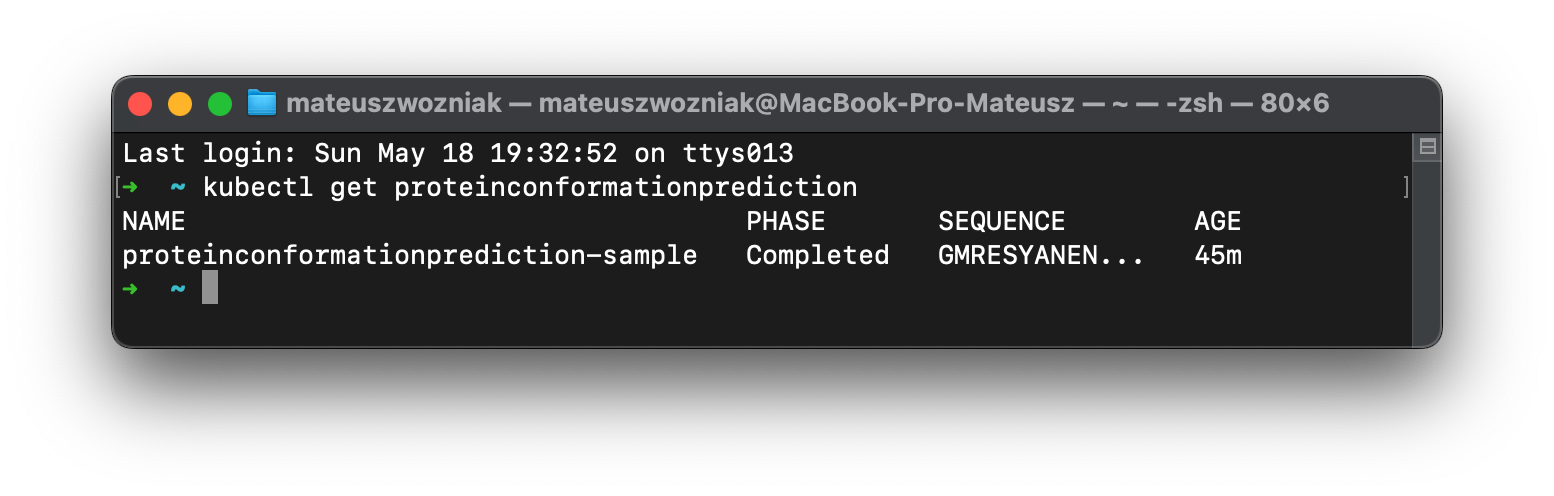
\includegraphics[width=\textwidth]{images/proteinconformationprediction_completed_terminal}
    \caption{Completed protein conformation prediction task}
    \label{fig:proteinconformationprediction_completed_terminal}
\end{figure}


\section{Comparison with manual AlphaFold installation}

To highlight the advantages of using the KubeFold operator, it is worth comparing the installation and execution process with the traditional manual approach required for AlphaFold.

\subsection{Traditional AlphaFold setup process}

Setting up AlphaFold manually requires numerous steps that demand significant technical expertise:

\begin{enumerate}
    \item \textbf{Environment preparation:} Install CUDA, cuDNN, and other GPU dependencies on a compatible machine.
    \item \textbf{Software installation:} Clone the AlphaFold repository, install Python dependencies, and configure the environment.
    \item \textbf{Database download:} Manually download multiple large databases.
    \item \textbf{Input preparation:} Format protein sequences according to AlphaFold requirements.
    \item \textbf{Execution configuration:} Configure GPU settings, memory allocation, and other runtime parameters.
    \item \textbf{Results management:} Manually collect, organize, and store prediction results.
    \item \textbf{Results sharing:} Set up a system to share results with team members.
\end{enumerate}

The entire process can take several days to complete, requiring expertise in Linux system administration, GPU configuration, Python environment management, and bioinformatics data handling.
Additionally, each step is prone to errors that can be difficult to troubleshoot.

\subsection{KubeFold approach}

In contrast, the KubeFold operator simplifies this process to just a few steps:

\begin{enumerate}
    \item Set up a Kubernetes cluster (can be automated using Cloud Infrastructure Formation software),
    \item Install the KubeFold operator,
    \item Create a \texttt{ProteinDatabase} resource,
    \item Create a \texttt{ProteinConformationPrediction} resource with the desired protein sequence.
\end{enumerate}

The entire setup and execution process that previously required days of work and specialized knowledge can be completed in hours with minimal Kubernetes expertise.
The operator handles all the complex tasks automatically:

\begin{itemize}
    \item Database provisioning and management
    \item Job scheduling across appropriate nodes
    \item Execution monitoring and status reporting
    \item Results storage and notification
\end{itemize}

This simplification makes protein structure prediction accessible to researchers without extensive computational expertise, allowing them to focus on their scientific work rather than infrastructure management.

\section{Computation artifacts overview}

After the computations were completed, the artifacts were sent to AWS S3 storage.
A directory was created in the bucket with a name containing the computation execution time, e.g., \texttt{default-proteinconformationprediction-sample\_20250518\_181911}.
The name also includes the Kubernetes resource name and namespace.
The directory contents are shown in screenshot~\ref{fig:bucket}.
The output directory contains several types of files that provide different aspects of the protein structure prediction:

\begin{itemize}
    \item \texttt{TERMS\_OF\_USE.md} - A markdown file containing the terms of use for AlphaFold predictions,
    \item \texttt{*\_model.cif} - The main output file containing the predicted 3D structure of the protein in CIF format, which can be visualized using molecular visualization software,
    \item \texttt{*\_confidences.json} - Detailed confidence scores for each residue in the predicted structure,
    \item \texttt{*\_summary\_confidences.json} - A condensed version of the confidence scores providing an overview of prediction reliability,
    \item \texttt{*\_ranking\_scores.csv} - A CSV file containing ranking scores for different model variants,
    \item \texttt{*\_data.json} - Additional metadata about the prediction run.
\end{itemize}

For each prediction run, AlphaFold generates multiple samples (in this case, 5 samples) to account for the stochastic nature of the prediction process.
Each sample is stored in its own subdirectory (e.g., \texttt{seed-1\_sample-0/}) and contains its own set of model files and confidence scores.
The final model file in the root directory represents the best prediction selected from all samples.

The \texttt{.cif} file allows visualization of the three-dimensional protein structure using software such as \textit{RCSB 3D View} (\url{https://www.rcsb.org/3d-view}).
An example visualization is shown in fig.~\ref{fig:protein_visualization}.

Additionally, an SMS message was sent to the user informing about the completed computation (see fig.~\ref{fig:sns_notification}).

\begin{figure}[htbp]
    \centering
    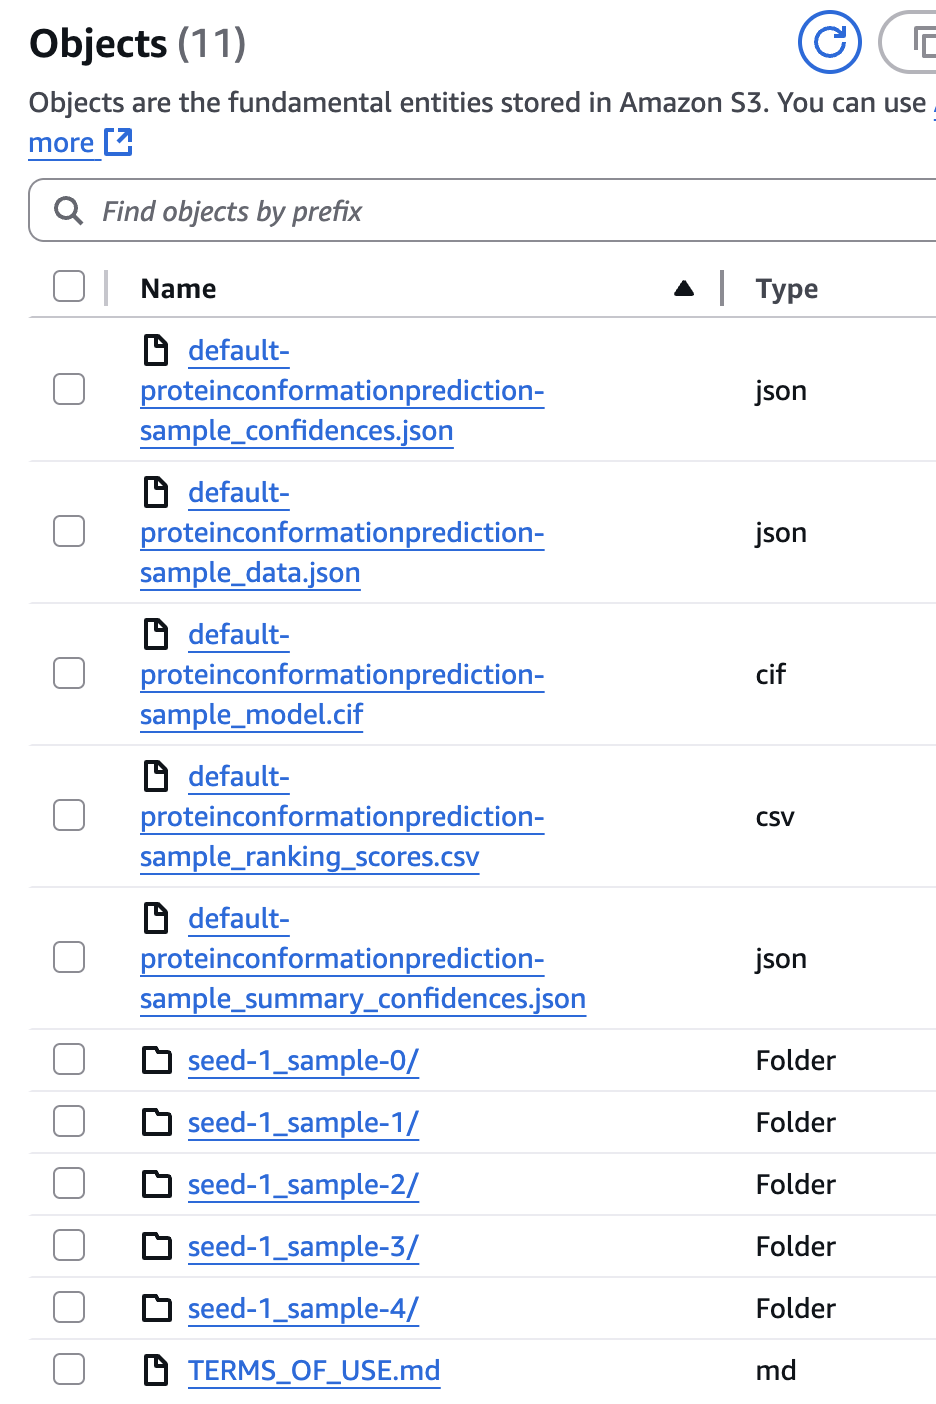
\includegraphics[width=\textwidth]{images/bucket2}
    \caption{Contents of bucket containg computation artifacts}
    \label{fig:bucket}
\end{figure}

\begin{figure}[htbp]
    \centering
    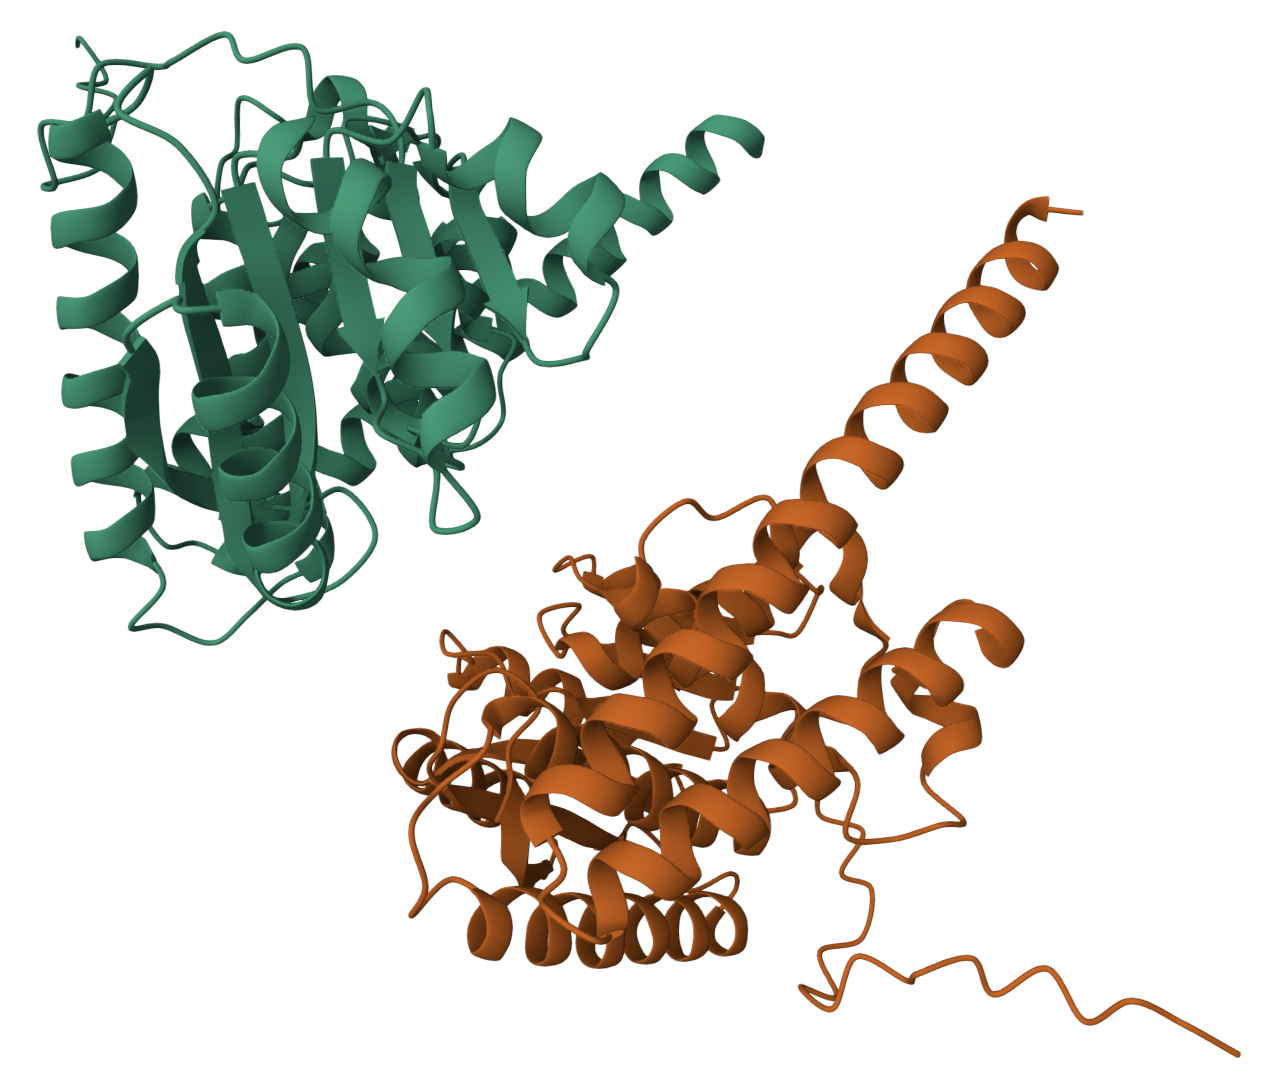
\includegraphics[width=\textwidth]{images/protein_visualization_small}
    \caption{Visualization of folded protein using RCSB visualization software \url{https://www.rcsb.org/3d-view}}
    \label{fig:protein_visualization}
\end{figure}

\begin{figure}[htbp]
    \centering
    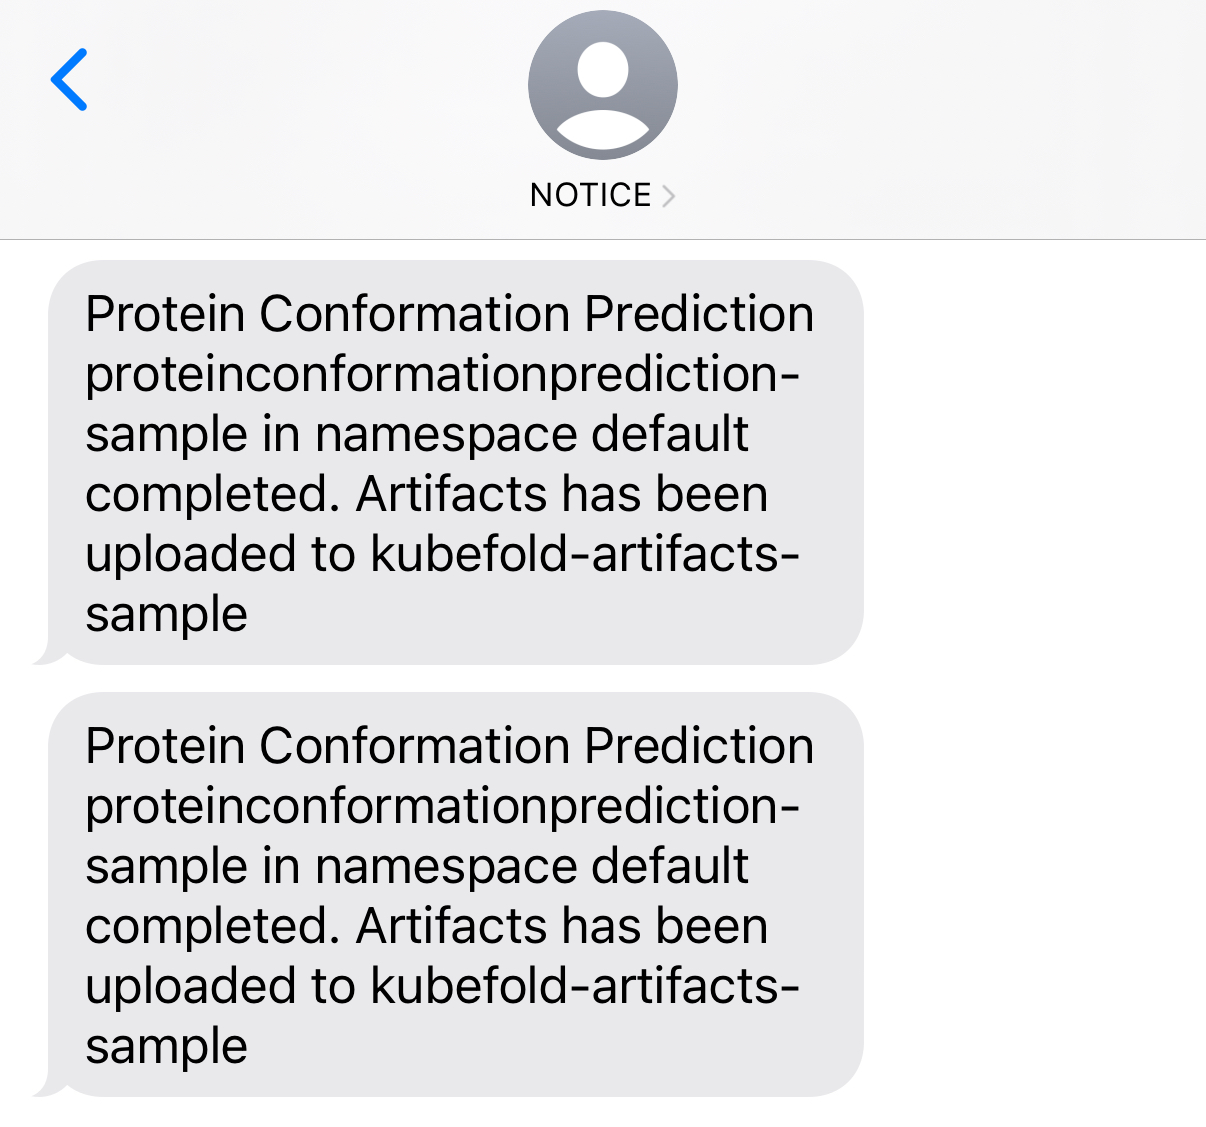
\includegraphics[width=\textwidth]{images/sns_notification_light}
    \caption{SMS Notification sent to research team member when computation is done}
    \label{fig:sns_notification}
\end{figure}

\section{Testing approach}

The KubeFold platform was tested using a manual testing approach. After implementing the operator and its components, the testing process involved creating a real Kubernetes cluster in AWS EKS, installing the operator, and running actual protein conformation predictions.

This end-to-end testing approach was chosen to validate the entire workflow in a production-like environment. The testing process followed these steps:

\begin{enumerate}
    \item Creating an AWS EKS cluster using the \texttt{eksctl} configuration described in listing~\ref{lst:eksctl}
    \item Installing the AWS FSx CSI Driver and configuring the \texttt{StorageClass}
    \item Deploying the KubeFold operator using the installation file
    \item Creating a \texttt{ProteinDatabase} custom resource and verifying the download process
    \item Creating a \texttt{ProteinConformationPrediction} custom resource and monitoring the prediction workflow
    \item Validating the output artifacts in AWS S3 storage
    \item Confirming the delivery of notifications via AWS SNS
\end{enumerate}

During testing, the operator's behavior was observed through Kubernetes logs and resource status updates. This approach allowed for direct verification of the operator's functionality in handling real-world scenarios, including error conditions and resource constraints.

The manual testing approach proved sufficient for validating the core functionality of the KubeFold platform. While unit tests and simulated cluster environments could provide additional validation layers, the end-to-end testing in a production environment offered the most comprehensive verification of the system's capabilities and integration with AWS services.
